\documentclass[DaoFP]{subfiles}
\begin{document}
    \setcounter{chapter}{8}

    \chapter{自然变换 (Natural Transformations)}

    我们已经看到,当两个对象$a$和$b$是同构的时,它们会在箭头集之间生成双射(bijections),我们现在可以将其表达为态射集(hom-sets)之间的同构(isomorphisms)。对于所有$x$,我们有:
    \begin{align*}
        \mathcal{C}(a, x) &\cong \mathcal{C}(b, x) \\
        \mathcal{C}(x, a) &\cong \mathcal{C}(x, b)
    \end{align*}
    但反过来并不成立。态射集之间的同构并不会导致对象之间的同构,除非满足附加的自然性条件(naturality conditions)。我们现在将在逐步更一般的设置中重新表述这些自然性条件。

    \section{态射函子之间的自然变换 (Natural Transformations Between Hom-Functors)}

    一种可以建立两个对象之间同构的方法是直接提供两个箭头,一个是另一个的逆。但通常情况下,更容易间接地完成,通过定义箭头之间的双射,无论是作用在两个对象上的箭头,还是从两个对象发出的箭头。

    例如,正如我们之前所看到的,对于每一个$x$,我们可能有一个可逆的箭头映射$\alpha_x$。
    \[
        \begin{tikzcd}
            \node(x) at (0, 2) {x};
            \node(a) at (-2, 0) {a};
            \node(b) at (2, 0) {b};
            \node(c1) at (-1, 1.5) {};
            \node(c2) at (-1.5, 1) {};
            \node(c3) at (-1, 2) {};
            \node(c4) at (-2, 1) {};
            \node(d1) at (1, 1.5) {};
            \node(d2) at (1.5, 1) {};
            \node(d3) at (1, 2) {};
            \node(d4) at (2, 1) {};
            \node (aa) at (-1, 0.75) {};
            \node (bb) at (1, 0.75) {};
            \draw[->] (x) .. controls (c1)  and (c2) .. (a); % bend
            \draw[->, green] (x) .. controls (c3)  and (c4) .. (a); % bend
            \draw[->, blue] (x) -- (a);
            \draw[->] (x) .. controls (d1)  and (d2) .. (b); % bend
            \draw[->, green] (x) .. controls (d3)  and (d4) .. (b); % bend
            \draw[->, blue] (x) -- (b);
            \draw[->, red, dashed] (aa) -- node[above]{\alpha_x} (bb);
        \end{tikzcd}
    \]
    换句话说,对于每一个$x$,存在一个态射集的映射:
    \[ \alpha_x \colon \mathcal{C}(x, a) \to \mathcal{C}(x, b) \]

    当我们变化$x$时,这两个态射集成为两个反变函子(contravariant functors),$\cat C(-, a)$和$\cat C(-, b)$,$\alpha$可以看作它们之间的一个映射。这样的函子映射,称为变换(transformation),实际上是一个个别映射$\alpha_x$的集合,每个$\mathcal{C}$中的对象$x$都有一个映射。

    函子$\mathcal{C}(-, a)$描述了世界如何看待$a$,而函子$\mathcal{C}(-, b)$描述了世界如何看待$b$。

    变换$\alpha$在这两个视角之间来回切换。$\alpha$的每个分量$\alpha_x$表明,从$x$看$a$的视角与从$x$看$b$的视角是同构的。

    我们之前讨论过的自然性条件(naturality condition)是:

    \[ \alpha_y \circ (- \circ g) = (- \circ g) \circ \alpha_x \]
    它将取自不同对象的$\alpha$的分量联系起来。换句话说,它将由箭头$g \colon y \to x$连接的两个观察者$x$和$y$的视角联系起来。

    这个方程的两边作用在态射集$\mathcal{C}(x, a)$上。结果位于态射集$\mathcal{C}(y, b)$中。我们可以将两边重写为:
    \begin{align*}
        \cat C(x, a) \xrightarrow{(- \circ g)} \cat C(y, a) \xrightarrow{\alpha_y} \cat C(y, b) \\
        \cat C(x, a) \xrightarrow{\alpha_x}  \cat C(x, b)  \xrightarrow{(- \circ g)}\cat C(y, b)
    \end{align*}

    与$g \colon y \to x$的预合成(precomposition)也是一个态射集的映射。实际上它是通过反变态射函子的提升(lifting)。我们可以将其分别写为$\mathcal{C}(g, a)$和$\mathcal{C}(g, b)$。
    \begin{align*}
        \cat C(x, a) \xrightarrow{\cat C(g, a)} \cat C(y, a) \xrightarrow{\alpha_y} \cat C(y, b) \\
        \cat C(x, a) \xrightarrow{\alpha_x}  \cat C(x, b)  \xrightarrow{\cat C(g, b)}\cat C(y, b)
    \end{align*}

    因此,自然性条件可以重写为:
    \[ \alpha_y \circ \mathcal{C}(g, a) = \mathcal{C}(g, b) \circ \alpha_x \]
    可以通过以下交换图来说明:
    \[
        \begin{tikzcd}
            \mathcal{C}(x, a)
            \arrow[d, "\alpha_x"]
            \arrow[r, "{\mathcal{C}(g, a)}"]
            &
            \mathcal{C}(y, a)
            \arrow[d, "\alpha_y"]
            \\
            \mathcal{C}(x, b)
            \arrow[r, "{\mathcal{C}(g, b)}"]
            & \mathcal{C}(y, b)
        \end{tikzcd}
    \]

    我们现在可以重新表述我们之前的结论:在满足自然性条件的情况下,函子$\mathcal{C}(-, a)$和$\mathcal{C}(-, b)$之间的可逆变换$\alpha$等价于$a$和$b$之间的同构。

    对于出射箭头(outgoing arrows),我们可以遵循完全相同的推理。这次我们从一个变换$\beta$开始,其分量为:
    \[ \beta_x \colon \mathcal{C}(a, x) \to \mathcal{C}(b, x) \]
    两个协变函子(covariant functors) $\mathcal{C}(a, -)$ 和 $\mathcal{C}(b, -)$ 分别描述了从$a$和$b$的角度看世界。可逆变换$\beta$告诉我们,这两个视角是等价的,而自然性条件
    \[ (g \circ -) \circ \beta_x = \beta_y \circ (g \circ -) \]
    告诉我们,当我们切换焦点时,它们的行为是良好的。

    下面的交换图说明了自然性条件:
    \[
        \begin{tikzcd}
            \mathcal{C}(a, x)
            \arrow[d, "\beta_x"]
            \arrow[r, "{\mathcal{C}(a, g)}"]
            &
            \mathcal{C}(a, y)
            \arrow[d, "\beta_y"]
            \\
            \mathcal{C}(b, x)
            \arrow[r, "{\mathcal{C}(b, g)}"]
            & \mathcal{C}(b, y)
        \end{tikzcd}
    \]

    同样,类似的可逆自然变换$\beta$可以建立$a$和$b$之间的同构。

    \section{函子之间的自然变换 (Natural Transformation Between Functors)}

    上一节中的两个态射函子是
    \begin{align*}
        F x &=   \mathcal{C}(a, x) \\
        G x &=   \mathcal{C}(b, x)
    \end{align*}
    它们都将范畴$\mathcal{C}$映射到集合范畴$\mathbf{Set}$,因为态射集都位于那里。我们可以说它们在$\mathbf{Set}$中创建了$\mathcal{C}$的两种不同的模型(models)。

    自然变换是两个这种模型之间的结构保持映射。
    \[
        \begin{tikzcd}
            && \cat C(a, x)
            \arrow[dd, "\beta_x"]
            \\
            x
            \arrow[rru, dashed, "{\cat C(a, -)}"]
            \arrow[rrd, dashed, "{\cat C(b, -)}"']
            \\
            && \cat C(b, x)
        \end{tikzcd}
    \]

    这个思想自然地扩展到任意一对范畴之间的函子。任何两个函子
    \begin{align*}
        F &\colon \mathcal{C} \to \mathcal{D} \\
        G &\colon \mathcal{C} \to \mathcal{D}
    \end{align*}
    可以被看作$\mathcal{D}$内$\mathcal{C}$的两个不同的模型。

    为了将一个模型转换为另一个模型,我们使用$\mathcal{D}$中的箭头来连接相应的点。对于$\mathcal{C}$中的每个对象$x$,我们选择一个箭头从$F x$到$G x$:
    \[ \alpha_x \colon F x \to G x \]
    因此,自然变换将对象映射到箭头。
    \[
        \begin{tikzcd}
            && F x
            \arrow[dd, "\alpha_x"]
            \\
            x
            \arrow[rru, dashed, "F"]
            \arrow[rrd, dashed, "G"']
            \\
            && G x
        \end{tikzcd}
    \]

    模型的结构既涉及对象,也涉及箭头,所以让我们看看箭头会发生什么。对于$\mathcal{C}$中的每个箭头$f \colon x \to y$,在$\mathcal{D}$中有两个相应的箭头:
    \begin{align*}
        F f &\colon F x \to F y \\
        G f &\colon G x \to G y
    \end{align*}
    这些是$f$的两个提升(liftings)。我们可以使用它们在每个模型的边界内移动。然后是$\alpha$的分量,它允许我们在模型之间切换。

    自然性条件(naturality)表明,无论你先在第一个模型内移动然后跳到第二个模型,还是先跳到第二个模型然后在其中移动,都不应该有区别。这通过交换的自然性方框(naturality square)来说明:

    \[
        \begin{tikzcd}
            F x
            \arrow[d, "\alpha_x"]
            \arrow[r, "F f"]
            &
            F y
            \arrow[d, "\alpha_y"]
            \\
            G x
            \arrow[r, "G f"]
            & G y
        \end{tikzcd}
    \]

    这样的满足自然性条件的箭头集合$\alpha_x$称为自然变换(natural transformation)。

    这是一个显示一对范畴、它们之间的两个函子和函子之间的自然变换$\alpha$的图:
    \[
        \begin{tikzcd}[column sep=huge]
            \mathcal{C}
            \arrow[bend left=50]{r}[name=U, label=above:$F$]{}
            \arrow[bend right=50]{r}[name=D, label=below:$G$]{}
            &
            \mathcal{D}
            \arrow[shorten <=10pt,shorten >=10pt,Rightarrow,to path={(U) -- node[label=left:$\alpha$] {} (D)}]{}
        \end{tikzcd}
    \]


    因为对于$\mathcal{C}$中的每个箭头都有一个对应的自然性方框,我们可以说自然变换将对象映射到箭头,将箭头映射到交换方框。

    如果一个自然变换的每个分量$\alpha_x$都是同构的,则称$\alpha$为自然同构(natural isomorphism)。

    我们现在可以重新陈述关于同构的主要结果:当且仅当在它们的态射函子之间存在自然同构时,两个对象是同构的(无论是协变的,还是反变的态射函子都可以)。

    自然变换提供了一种非常方便的高级方式,用于在各种情况下表达交换条件。我们将在此基础上重新表述代数数据类型(algebraic data types)的定义。

    \section{编程中的自然变换 (Natural Transformations in Programming)}

    自然变换是一组由对象参数化的箭头。在编程中,这对应于由类型参数化的函数族,也就是多态函数(polymorphic function)。

    自然变换参数的类型由一个函子描述,返回类型由另一个函子描述。

    在Haskell中,我们可以定义一个接受两个类型构造器表示两个函子的自然变换数据类型:

    \begin{haskell}
        data Natural :: (Type -> Type) -> (Type -> Type) -> Type where
        Natural :: (forall a. f a -> g a) -> Natural f g
    \end{haskell}
    \hask{forall}量词告诉编译器,这个函数是多态的——也就是说,它针对每种类型\hask{a}定义。只要\hask{f}和\hask{g}是函子,这个公式就定义了一个自然变换。

    但是\hask{forall}定义的类型非常特殊。它们在\index{参数多态性(parametric polymorphism)}\emph{参数多态性}的意义上是多态的。这意味着同一个公式适用于所有类型。我们已经看到了身份函数(identity function)的例子,可以写为:
    \begin{haskell}
        id :: forall a. a -> a
        id x = x
    \end{haskell}
    这个函数体非常简单,就是变量\hask{x}。无论\hask{x}的类型是什么,公式保持不变。

    这与\index{临时多态性(ad-hoc polymorphism)}\emph{临时多态性}形成对比。临时多态性函数可以对不同的类型使用不同的实现。一个这样的函数的例子是\hask{fmap},它是\hask{Functor}类型类的成员函数。对于列表有一个\hask{fmap}的实现,对于\hask{Maybe}有一个不同的实现,依此类推,每种情况各自实现。

    在Haskell中,标准的(参数多态)自然变换的定义使用了一个类型同义词(type synonym):
    \begin{haskell}
        type Natural f g = forall a. f a -> g a
    \end{haskell}
    \index{\hask{type} synonym}\hask{type}声明引入了一个别名,作为右侧的简写。

    事实证明,将自然变换的类型限制为参数多态性会产生深远的影响。这样的函数自动满足自然性条件。这是一个\index{参数性(parametricity)}参数性自动生成所谓\index{免费定理(theorems for free)}\emph{免费定理}的例子。

    我们不能在Haskell中表达箭头的等式,但我们可以使用自然性来转换程序。特别是,如果\hask{alpha}是一个自然变换,我们可以将:
    \begin{haskell}
        fmap h . alpha
    \end{haskell}
    替换为:
    \begin{haskell}
        alpha . fmap h
    \end{haskell}
    在这里,编译器会自动判断应该使用哪个版本的\hask{fmap}和\hask{alpha}的哪个分量。

    我们还可以使用更高级的语言选项来显式地做出选择。我们可以使用一对函数来表达自然性:
    \begin{haskell}
        oneWay ::
        forall f g a b. (Functor f, Functor g) =>
        Natural f g -> (a -> b) -> f a -> g b
        oneWay alpha h = fmap @g h . alpha @a
    \end{haskell}
    \begin{haskell}
        otherWay ::
        forall f g a b. (Functor f, Functor g) =>
        Natural f g -> (a -> b) -> f a -> g b
        otherWay alpha h = alpha @b . fmap @f h
    \end{haskell}
    注释\hask{@a}和\hask{@b}指定了参数多态函数\hask{alpha}的分量,注释\hask{@f}和\hask{@g}指定了为其实例化的临时多态\hask{fmap}的函子。

    文件顶部需要指定以下Haskell扩展:
    \begin{haskell}
    {-# language RankNTypes #-}
    {-# language TypeApplications #-}
    {-# language ScopedTypeVariables #-}
    \end{haskell}

    以下是一个有用的函数例子,它是列表函子和\hask{Maybe}函子之间的自然变换:
    \begin{haskell}
        safeHead :: Natural [] Maybe
        safeHead [] = Nothing
        safeHead (a : as) = Just a
    \end{haskell}
    (标准库中的\hask{head}函数是不安全的,因为它在给定空列表时会出错。)

    另一个例子是\hask{reverse}函数,它反转一个列表。它是列表函子到列表函子的自然变换:
    \begin{haskell}
        reverse :: Natural [] []
        reverse [] = []
        reverse (a : as) = reverse as ++ [a]
    \end{haskell}
    顺便说一下,这是一个非常低效的实现。实际的库函数使用了优化的算法。

    理解自然变换的一个有用直觉是建立在函子像数据容器(container)的想法之上的。对于一个容器,有两种完全正交的操作:你可以转换它包含的数据,而不改变容器的形状。这就是\hask{fmap}所做的事情。或者你可以在不修改数据的情况下,将数据转移到另一个容器中。这就是自然变换所做的事情:它是将“东西”在容器之间移动,而不知道“东西”是什么的过程。

    换句话说,自然变换将一个容器的内容重新打包到另一个容器中。它以与内容类型无关的方式进行,这意味着它不能检查、创建或修改内容。它所能做的只是将其移动到新位置,或将其丢弃。

    自然性条件强制了这两种操作的正交性。无论你是先修改数据然后将其移动到另一个容器中,还是先移动它,然后修改,都没有关系。

    这是另一个成功将复杂问题分解为一系列更简单问题的例子。不过请记住,并不是每个包含数据的容器操作都可以这样分解。例如,过滤操作需要既检查数据,又改变容器的大小甚至形状。

    另一方面,几乎每个参数多态函数都是自然变换。在某些情况下,你可能需要考虑恒等函子(identity functor)或常量函子(constant functor)作为源或目标。例如,参数多态的恒等函数可以被视为两个恒等函子之间的自然变换。

    \subsection{自然变换的垂直组合 (Vertical Composition of Natural Transformations)}

    自然变换只能在\emph{平行}函子之间定义,也就是说,这些函子共享相同的源范畴和相同的目标范畴。这种平行函子形成了一个函子范畴(functor category)。两个范畴$\mathcal{C}$和$\mathcal{D}$之间的函子范畴的标准表示是$[\mathcal{C}, \mathcal{D}]$。你只需将两个范畴的名称放在方括号之间。

    $[\mathcal{C}, \mathcal{D}]$中的对象是函子,箭头是自然变换。

    为了证明这确实是一个范畴,我们必须定义自然变换的组合。当我们记住自然变换的分量是目标范畴中的常规箭头时,这很容易。这些箭头是可组合的。

    确实,假设我们有一个从函子$F$到$G$的自然变换$\alpha$。我们想要将其与另一个从$G$到$H$的自然变换$\beta$组合。

    \[
        \begin{tikzcd}[column sep=huge]
            \mathcal{C}
            \arrow[bend left=60]{rr}[name=U, label=above:$F$]{}
            \arrow[]{rr}[name=M, label={[xshift=15pt, yshift=-5pt]:$G$}]{}
            \arrow[bend right=60]{rr}[name=D, label=below:$H$]{}
            &&
            \mathcal{D}
            \arrow[shorten <=8pt, shorten >=8pt,Rightarrow, to path={(U) -- node[label=left:$\alpha$] {} (M)}]{}
            \arrow[shorten <=8pt, shorten >=8pt,Rightarrow, to path={(M) -- node[label=left:$\beta$] {} (D)}]{}
        \end{tikzcd}
    \]

    让我们看看这些变换在某个对象$x$处的分量
    \[ \alpha_x \colon F \, x \to G \, x \]
    \[ \beta_x \colon G \, x \to H \, x \]
    这些仅仅是$\mathcal{D}$中的两个箭头,它们是可组合的。因此,我们可以如下定义一个复合自然变换$\gamma$:
    \[ \gamma \colon F \to H\]
    \[ \gamma_x = \beta_x \circ \alpha_x \]
    这被称为自然变换的\emph{垂直组合}(vertical composition)。你会看到它写作点$\gamma = \beta \cdot \alpha$或简单的并置$\gamma = \beta \alpha$。

    可以通过将两个自然性方框垂直粘合在一起证明$\gamma$的自然性条件:
    \[
        \begin{tikzcd}
            F x
            \arrow[d, "\alpha_x"]
            \arrow[r, "F f"]
            \arrow[dd, bend right = 60, "\gamma_x"']
            &
            F y
            \arrow[d, "\alpha_y"]
            \arrow[dd, bend left = 60, "\gamma_y"]
            \\
            G x
            \arrow[r, "G f"]
            \arrow[d, "\beta_x"]
            & G y
            \arrow[d, "\beta_y"]
            \\
            H x
            \arrow[r, "H f"]
            & H y
        \end{tikzcd}
    \]

    在Haskell中,自然变换的垂直组合只是应用于多态函数的常规函数组合。使用自然变换在容器之间移动项目的直觉,垂直组合将两个这样的移动组合在一起,一个接一个地进行。

    \subsection{函子范畴 (Functor Categories)}

    由于自然变换的组合是根据箭头的组合定义的,因此它是自动关联的。

    还有一个恒等自然变换$id_F$,它定义在每个函子$F$上。它在$x$处的分量是对象$F x$处的常规恒等箭头:
    \[ (id_F)_x = id_{F x} \]

    总结一下,对于每一对范畴$\mathcal{C}$和$\mathcal{D}$,都有一个函子范畴$[\mathcal{C}, \mathcal{D}]$,其箭头为自然变换。

    在该范畴中的态射集是两个函子$F$和$G$之间的自然变换集合。按照标准的符号表示方式,我们将其写为:
    \[ [\mathcal{C}, \mathcal{D}](F, G) \]
    范畴的名称后面跟着两个对象(在这里是函子)的名称,用括号括起来。

    在范畴论中,对象和箭头的表示不同。对象是点,箭头是有尖头的线。

    在$\mathbf{Cat}$,即范畴的范畴中,函子被表示为箭头。但在一个函子范畴$[\cat C, \cat D]$中,函子是点,自然变换是箭头。

    在一个范畴中的箭头在另一个范畴中可能是一个对象。

    \begin{exercise}
        证明自然变换复合的自然性条件:
        \[ \gamma_y \circ F f = H f \circ \gamma_x \]
        提示:使用$\gamma$的定义以及$\alpha$和$\beta$的两个自然性条件。
    \end{exercise}

    \subsection{自然变换的水平组合 (Horizontal Composition of Natural Transformations)}

    自然变换的第二种组合方式是由函子组合引起的。假设我们有一对可组合的函子
    \begin{align*}
        F \colon \mathcal{C} \to \mathcal{D}
        &&G \colon \mathcal{D} \to \mathcal{E}
    \end{align*}
    同时,还有另一对可组合的函子:
    \begin{align*}
        F' \colon \mathcal{C} \to \mathcal{D}
        && G' \colon \mathcal{D} \to \mathcal{E}
    \end{align*}
    我们还拥有两个自然变换:
    \begin{align*}
        \alpha \colon F \to F'
        && \beta \colon G \to G'
    \end{align*}
    图示如下:
    \[
        \begin{tikzcd}[column sep=huge]
            \mathcal{C}
            \arrow[bend left=50]{r}[name=U, label=above:$F$]{}
            \arrow[bend right=50]{r}[name=D, label=below:$F'$]{}
            &
            \mathcal{D}
            \arrow[bend left=50]{r}[name=U1, label=above:$G$]{}
            \arrow[bend right=50]{r}[name=D1, label=below:$G'$]{}
            &
            \mathcal{E}
            \arrow[shorten <=10pt,shorten >=10pt,Rightarrow,to path={(U) -- node[label=left:$\alpha$] {} (D)}]{}
            \arrow[shorten <=10pt,shorten >=10pt,Rightarrow,to path={(U1) -- node[label=left:$\beta$] {} (D1)}]{}
        \end{tikzcd}
    \]
    水平组合$\beta \circ \alpha$将$G \circ F$映射到$G' \circ F'$。
    \[
        \begin{tikzcd}[column sep=huge]
            \mathcal{C}
            \arrow[bend left=50]{r}[name=U, label=above:$G \circ F$]{}
            \arrow[bend right=50]{r}[name=D, label=below:$G' \circ F'$]{}
            &
            \mathcal{E}
            \arrow[shorten <=10pt,shorten >=10pt,Rightarrow,to path={(U) -- node[label=left:$\beta \circ \alpha$] {} (D)}]{}
        \end{tikzcd}
    \]

    让我们选择$\mathcal{C}$中的一个对象$x$,并尝试定义复合变换$(\beta \circ \alpha)$在$x$处的分量。它应该是$\mathcal{E}$中的一个态射:
    \[ (\beta \circ \alpha)_x \colon G ( F x) \to G' ( F' x) \]

    我们可以使用$\alpha$将$x$映射到一个箭头
    \[ \alpha_x \colon F x \to F' x \]
    我们可以用$G$提升这个箭头
    \[ G (\alpha_x) \colon G (F x) \to G (F' x) \]
    要从这里到达$G' (F' x)$,我们可以使用$\beta$的适当分量
    \[ \beta_{F' x} \colon G (F' x) \to G' (F' x) \]
    总之,我们有
    \[ (\beta \circ \alpha)_x = \beta_{F' x} \circ G (\alpha_x) \]

    但还有另一个同样合理的候选人:
    \[ (\beta \circ \alpha)_x = G'(\alpha_x) \circ \beta_{F x}\]
    幸运的是,由于$\beta$的自然性,它们是相等的。

    \[
        \begin{tikzcd}
            && G(F x)
            \arrow[dd, red, "G(\alpha_x)"]
            \arrow[dr, blue, "\beta_{F x}"]
            \\
            & F x
            \arrow[rr, bend right=10, dashed, gray]
            \arrow[ur, bend right=10, dashed]
            \arrow[dd, red, "\alpha_x"]
            && G' (F x)
            \arrow[dd, red, "G'(\alpha_x)"]
            \\
            x
            \arrow[ur, dashed]
            \arrow[dr, gray, dashed]
            && G(F' x)
            \arrow[dr, blue, "\beta_{F' x}"]
            \\
            &F' x
            \arrow[rr, bend right=10, dashed, gray]
            \arrow[ur, bend right=10, dashed]
            && G'(F' x)
        \end{tikzcd}
    \]
    自然性条件的证明留给有志的读者作为练习。

    我们可以直接将其转换为Haskell。我们从两个自然变换开始:
    \begin{haskell}
        alpha :: forall x. F x -> F' x
        beta  :: forall x. G x -> G' x
    \end{haskell}
    它们的水平组合有以下类型签名:
    \begin{haskell}
        beta_alpha :: forall x. G (F x) -> G' (F' x)
    \end{haskell}
    它有两个等价的实现。第一个是:
    \begin{haskell}
        beta_alpha = beta . fmap alpha
    \end{haskell}
    编译器将自动选择正确版本的\hask{fmap},即适用于函子\hask{G}的版本。第二个实现是:
    \begin{haskell}
        beta_alpha = fmap alpha . beta
    \end{haskell}
    在这里,编译器将选择\hask{fmap}的版本,适用于函子\hask{G'}。

    水平组合的直觉是什么?我们之前已经看到,自然变换可以被看作是数据在两个容器(函子)之间的重新打包。在这里,我们处理的是嵌套容器。我们从由\hask{G}描述的外部容器开始,该容器中填充了由\hask{F}描述的内部容器。我们有两个自然变换,\hask{alpha}用于将\hask{F}的内容传输到\hask{F'},\hask{beta}用于将\hask{G}的内容移动到\hask{G'}。有两种方法可以将数据从\hask{G (F x)}移动到\hask{G'(F' x)}。我们可以使用\hask{fmap alpha}来重新打包所有内部容器,然后使用\hask{beta}来重新打包外部容器。

    \[
        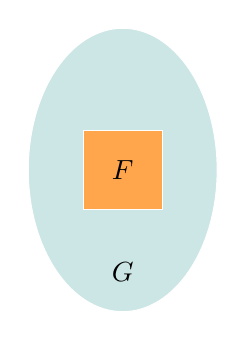
\begin{tikzpicture}
            \filldraw[fill=blue!50!green!20, draw=white] (0, 0) ellipse (1.2 and 1.8);
            \filldraw[fill=orange!70, draw=white] (-0.5, -0.5) rectangle (0.5, 0.5);
            \node at (0, 0) {$F$};
            \node at (0, -1.3) {$G$};
        \end{tikzpicture}
        \hspace{20pt}
        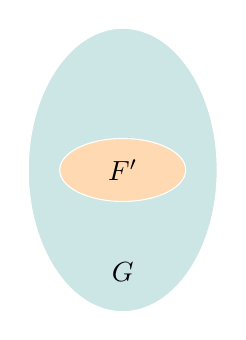
\begin{tikzpicture}
            \filldraw[fill=blue!50!green!20, draw=white] (0, 0) ellipse (1.2 and 1.8);
            \filldraw[fill=orange!30, draw=white] (0, 0) ellipse (0.8 and 0.4);
            \node at (0, 0) {$F'$};
            \node at (0, -1.3) {$G$};
        \end{tikzpicture}
        \hspace{20pt}
        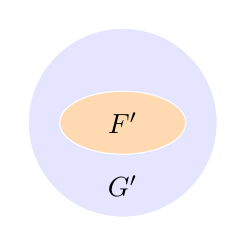
\begin{tikzpicture}
            \filldraw[fill=blue!10, draw=white] (0, 0) circle (1.2);
            \filldraw[fill=orange!30, draw=white] (0, 0) ellipse (0.8 and 0.4);
            \node at (0, 0) {$F'$};
            \node at (0, -0.8) {$G'$};
        \end{tikzpicture}
    \]


    或者我们可以先使用\hask{beta}来重新打包外部容器,然后应用\hask{fmap alpha}来重新打包所有内部容器。最终结果是相同的。

    \[
        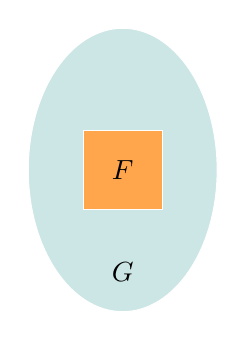
\begin{tikzpicture}
            \filldraw[fill=blue!50!green!20, draw=white] (0, 0) ellipse (1.2 and 1.8);
            \filldraw[fill=orange!70, draw=white] (-0.5, -0.5) rectangle (0.5, 0.5);
            \node at (0, 0) {$F$};
            \node at (0, -1.3) {$G$};
        \end{tikzpicture}
        \hspace{20pt}
        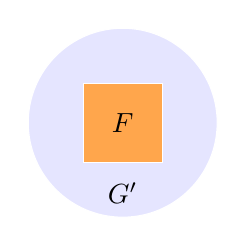
\begin{tikzpicture}
            \filldraw[fill=blue!10, draw=white] (0, 0) circle (1.2);
            \filldraw[fill=orange!70, draw=white] (-0.5, -0.5) rectangle (0.5, 0.5);
            \node at (0, 0) {$F$};
            \node at (0, -0.9) {$G'$};
        \end{tikzpicture}
        \hspace{20pt}
        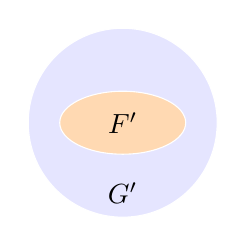
\begin{tikzpicture}
            \filldraw[fill=blue!10, draw=white] (0, 0) circle (1.2);
            \filldraw[fill=orange!30, draw=white] (0, 0) ellipse (0.8 and 0.4);
            \node at (0, 0) {$F'$};
            \node at (0, -0.9) {$G'$};
        \end{tikzpicture}
    \]


    \begin{exercise}
        实现\hask{safeHead}和\hask{reverse}的水平组合的两个版本。比较它们在各种参数上的作用。
    \end{exercise}

    \begin{exercise}
        同样做\hask{reverse}和\hask{safeHead}的水平组合。
    \end{exercise}

    \subsection{Whiskering}

    水平组合经常在其中一个自然变换是恒等变换时使用。这种组合有一个简写表示法。例如,$\alpha \circ id_F$写作$\alpha \circ F$。

    由于图的特征形状,这种组合被称为“Whiskering”。
    \[
        \begin{tikzcd}[column sep=huge]
            \mathcal{C}
            \arrow[r, "F"]
            &
            \mathcal{D}
            \arrow[bend left=50]{r}[name=U1, label=above:$G$]{}
            \arrow[bend right=50]{r}[name=D1, label=below:$G'$]{}
            &
            \mathcal{E}
            \arrow[shorten <=10pt,shorten >=10pt,Rightarrow,to path={(U1) -- node[label=left:$\alpha$] {} (D1)}]{}
        \end{tikzcd}
    \]
    在分量中,我们有:
    \[ (\alpha \circ F)_x = \alpha_{F x} \]

    让我们考虑如何将其翻译为Haskell。自然变换是一个多态函数。由于参数性,它对所有类型都是由同一个公式定义的。因此在右边Whiskering不会改变公式,它改变了函数签名。

    例如,如果这是\hask{alpha}的声明:
    \begin{haskell}
        alpha :: forall x. G x -> G' x
    \end{haskell}
    那么它的Whiskering版本将是:
    \begin{haskell}
        alpha_f :: forall x. G (F x) -> G' (F x)
        alpha_f = alpha
    \end{haskell}
    由于Haskell的类型推导,这种转换是隐式的。当调用一个多态函数时,我们不必指定执行自然变换的哪个分量——类型检查器会通过查看参数的类型来判断。

    此时的直觉是我们重新打包外部容器而保留内部容器不变。

    类似地,$id_H \circ \alpha$写作$H \circ \alpha$。
    \[
        \begin{tikzcd}[column sep=huge]
            \mathcal{D}
            \arrow[bend left=50]{r}[name=U, label=above:$G$]{}
            \arrow[bend right=50]{r}[name=D, label=below:$G'$]{}
            &
            \mathcal{E}
            \arrow[r, "H"]
            &
            \mathcal{F}
            \arrow[shorten <=10pt,shorten >=10pt,Rightarrow,to path={(U) -- node[label=left:$\alpha$] {} (D)}]{}
        \end{tikzcd}
    \]
    在分量中:
    \[(H \circ \alpha)_x = H (\alpha_x) \]

    在Haskell中,通过$H$提升$\alpha_x$是用\hask{fmap}完成的,因此给定:
    \begin{haskell}
        alpha :: forall x. G x -> G' x
    \end{haskell}
    Whiskering版本将是:
    \begin{haskell}
        h_alpha :: forall x. H (G x) -> H (G' x)
        h_alpha = fmap alpha
    \end{haskell}
    同样,Haskell的类型推导引擎会判断使用哪个版本的\hask{fmap}(在这里,它是\hask{Functor}实例\hask{G}的那个)。

    直觉上,这表明我们重新打包了内部容器的内容,同时保留外部容器不变。

    最后,在许多应用中,自然变换在两侧都进行了Whiskering:
    \[
        \begin{tikzcd}[column sep=huge]
            \mathcal{C}
            \arrow[r, "F"]
            &
            \mathcal{D}
            \arrow[bend left=50]{r}[name=U1, label=above:$G$]{}
            \arrow[bend right=50]{r}[name=D1, label=below:$G'$]{}
            &
            \mathcal{E}
            \arrow[shorten <=10pt,shorten >=10pt,Rightarrow,to path={(U1) -- node[label=left:$\alpha$] {} (D1)}]{}
            \arrow[r, "H"]
            &
            \mathcal{F}
        \end{tikzcd}
    \]
    在分量中,我们有:
    \[ (H \circ \alpha \circ F) x = H (\alpha_{F x})\]
    在Haskell中:
    \begin{haskell}
        h_alpha_f :: forall x. H (G (F x)) -> H (G' (F x))
        h_alpha_f = fmap alpha
    \end{haskell}

    这里的直觉是我们有一个三层容器;我们正在重新排列中间层,同时保留外层容器和所有内层容器不变。

    \subsection{交换律 (Interchange Law)}

    我们可以将垂直组合与水平组合结合起来,如下图所示:
    \[
        \begin{tikzcd}[column sep=huge]
            \mathcal{C}
            \arrow[bend left=60]{rr}[name=U, label=above:$F$]{}
            \arrow[]{rr}[name=M, label={[xshift=15pt, yshift=-5pt]:$G$}]{}
            \arrow[bend right=60]{rr}[name=D, label=below:$H$]{}
            &&
            \mathcal{D}
            \arrow[bend left=60]{rr}[name=U1, label=above:$F'$]{}
            \arrow[]{rr}[name=M1, label={[xshift=15pt, yshift=-5pt]:$G'$}]{}
            \arrow[bend right=60]{rr}[name=D1, label=below:$H'$]{}
            &&
            \mathcal{E}
            \arrow[shorten <=8pt, shorten >=8pt,Rightarrow, to path={(U) -- node[label=left:$\alpha$] {} (M)}]{}
            \arrow[shorten <=8pt, shorten >=8pt,Rightarrow, to path={(M) -- node[label=left:$\beta$] {} (D)}]{}
            \arrow[shorten <=8pt, shorten >=8pt,Rightarrow, to path={(U1) -- node[label=left:$\alpha'$] {} (M1)}]{}
            \arrow[shorten <=8pt, shorten >=8pt,Rightarrow, to path={(M1) -- node[label=left:$\beta'$] {} (D1)}]{}
        \end{tikzcd}
    \]
    交换律(Interchange law)规定组合的顺序并不重要:我们可以先做垂直组合,然后是水平组合;或者先做水平组合,然后是垂直组合。

\end{document}


\section{重访泛在构造 (Universal Constructions Revisited)}

老子说,最简单的模式是最清晰的。

我们已经看到了和、积、指数、自然数和列表的定义。

传统的定义这些数据类型的方法是探索它们的内部。这是集合论的方式:我们考察新集合的元素如何从旧集合的元素构造出来。一个和的元素要么是第一个集合的元素,要么是第二个集合的元素。一个积的元素是一对元素,依此类推。从工程的角度来看,我们是在观察对象。

在范畴论中,我们采取相反的方法。我们不关心对象的内部或它是如何实现的。我们关心的是对象的目的,它如何被使用,以及它如何与其他对象交互。我们从实用主义的角度看待对象。

这两种方法各有其优点。范畴论的方法出现较晚,因为你需要研究大量的实例才能看清楚模式。但一旦你看到了这些模式,你就会发现事物之间意想不到的联系,比如和与积之间的对偶性。

通过它们之间的联系来定义特定的对象需要考察它们可能与之交互的无限多个对象。

“告诉我你与宇宙的关系,我就会告诉你是谁。”

通过关于范畴中所有对象的映射来定义对象的过程被称为“泛在构造 (universal construction)”。

为什么自然变换 (natural transformations) 如此重要?这是因为大多数范畴构造涉及交换图 (commuting diagrams)。如果我们可以将这些图重构为自然性方块 (naturality squares),我们就能在抽象的阶梯上更进一步,并获得新的有价值的见解。

能够将大量的事实压缩成简洁优雅的公式,有助于我们发现新的模式。例如,我们会看到同态集之间的自然同构在范畴论中随处可见,最终引出了伴随 (adjunction) 的概念。

但首先,我们将详细研究几个例子,以了解范畴论简洁语言的含义。例如,我们将尝试解码这样的陈述:两个对象的和(或称余积)由以下自然同构定义:

\[
    [\mathbf{2}, \mathcal{C}](D, \Delta_x) \cong \mathcal{C}(a + b, x)
\]

\subsection{选择对象 (Picking objects)}

即使是指向一个对象这样简单的任务,在范畴论中也有特殊的解释。我们已经看到,指向一个集合的元素等同于从单元素集合中选择一个函数。同样,在范畴中选择一个对象等同于从单对象范畴中选择一个函子。或者,可以通过从另一个范畴中的常值函子 (constant functor) 来完成。

我们经常想要选择一对对象。这也可以通过从一个双对象的简图范畴中选择一个函子来完成。同样,选择一个箭头等同于从“行走箭头 (walking arrow)”范畴中选择一个函子,等等。

通过明智地选择我们的函子和它们之间的自然变换,我们可以重新表述到目前为止我们看到的所有泛在构造。

\subsection{作为自然变换的余脚 (Cospans as natural transformations)}

和的定义要求选择两个需要求和的对象;以及一个第三对象作为映射出去的目标。

\[
    \begin{tikzcd}
        a
        \arrow[dr, bend left, "\text{Left}"']
        \arrow[ddr, bend right, "f"']
        && b
        \arrow[dl, bend right, "\text{Right}"]
        \arrow[ddl, bend left, "g"]
        \\
        &a + b
        \arrow[d, dashed, "h"]
        \\
        & c
    \end{tikzcd}
\]

这个图可以进一步分解为两个更简单的形状,称为“余脚 (cospans)”:

\[
    \begin{tikzcd}
        a
        \arrow[dr, ""']
        && b
        \arrow[dl, ""]
        \\
        & x
    \end{tikzcd}
\]

要构造一个余脚,我们首先要选择一对对象。为此,我们从一个双对象范畴 $\mathbf{2}$ 开始。我们将其对象称为 $1$ 和 $2$。我们使用一个函子
\[ D \colon \mathbf{2} \to \mathcal{C} \]
来选择对象 $a$ 和 $b$:
\begin{align*}
    D\, 1 &= a \\
    D\, 2 &= b
\end{align*}
($D$ 代表“图 (diagram)”,因为这两个对象在 $\mathcal{C}$ 中形成了一个非常简单的由两个点组成的图。)

我们使用常值函子 (constant functor)
\[ \Delta_x \colon \mathbf{2} \to \mathcal{C} \]
来选择对象 $x$。这个函子将 $1$ 和 $2$ 都映射到 $x$(并将两个恒等箭头映射到 $id_x$)。

由于这两个函子都从 $\mathbf{2}$ 到 $\mathcal{C}$,我们可以在它们之间定义一个自然变换 $\alpha$。在这种情况下,它只是两个箭头的组合:
\begin{align*}
    \alpha_1 \colon D \, 1 \to \Delta_x 1 \\
    \alpha_2 \colon D \, 2 \to \Delta_x 2
\end{align*}
这些正是余脚中的两个箭头。

由于 $\mathbf{2}$ 中没有箭头(除了恒等箭头),所以 $\alpha$ 的自然性条件是显而易见的。

可能有许多余脚共享相同的三个对象——这意味着:在两个函子 $D$ 和 $\Delta_x$ 之间可能有许多自然变换。这些自然变换在函子范畴 $[\mathbf{2}, \mathcal{C}]$ 中形成了一个同态集,即:
\[ [\mathbf{2}, \mathcal{C}](D, \Delta_x) \]

\subsection{余脚的函子性 (Functoriality of cospans)}

让我们考虑当我们开始在余脚中改变对象 $x$ 时会发生什么。我们有一个映射 $F$,它将 $x$ 映射到 $x$ 上的余脚集合:
\[ F x = [\mathbf{2}, \mathcal{C}](D, \Delta_x) \]
这个映射在 $x$ 上表现为函子性。

要看到这一点,请考虑一个箭头 $m \colon x \to y$。这个箭头的提升是两个自然变换集合之间的映射:
\[ [\mathbf{2}, \mathcal{C}](D, \Delta_x) \to [\mathbf{2}, \mathcal{C}](D, \Delta_{y}) \]

这看起来可能非常抽象,直到你记住自然变换有分量,这些分量只是普通的箭头。左侧集合的一个元素是一个自然变换:
\[ \mu \colon D \to \Delta_x \]
它有两个对应于 $\mathbf{2}$ 中两个对象的分量。例如,我们有:
\[ \mu_1 \colon D \, 1 \to \Delta_x 1 \]
或者,使用 $D$ 和 $\Delta$ 的定义:
\[ \mu_1 \colon a \to x \]
这只是我们余脚的左腿。

同样,右侧集合的元素是一个自然变换:
\[ \nu \colon D \to \Delta_{y} \]
它在 $1$ 处的分量是一个箭头:
\[ \nu_1 \colon a \to y \]
我们可以通过将其与 $m \colon x \to y$ 后组合来从 $\mu_1$ 到 $\nu_1$。因此,$m$ 的提升是一个逐分量后组合 $(m \circ -)$:
\begin{align*}
    \nu_1 = m \circ \mu_1 \\
\end{align*}
\begin{align*}
    \nu_2 = m \circ \mu_2
\end{align*}

\subsection{和作为泛在余脚 (Sum as a universal cospan)}

在你可以在对 $a$ 和 $b$ 进行构造的所有余脚中,我们称为 $\text{Left}$ 和 $\text{Right}$ 的箭头在 $a + b$ 上汇聚的那个是非常特殊的。有一个唯一的映射从它映射到任何其他余脚——一个使两个三角形交换的映射。
\[
    \begin{tikzcd}
        a
        \arrow[dr, bend left, "\text{Left}"']
        \arrow[ddr, bend right, "f"']
        && b
        \arrow[dl, bend right, "\text{Right}"]
        \arrow[ddl, bend left, "g"]
        \\
        &a + b
        \arrow[d, dashed, "h"]
        \\
        & x
    \end{tikzcd}
\]

我们现在能够将这种条件转换为关于自然变换和同态集的陈述。箭头 $h$ 是同态集 $\mathcal{C}(a + b, x)$ 的元素。

$x$ 上的余脚是一个自然变换,即函子范畴中的同态集的元素:
\[ [\mathbf{2}, \mathcal{C}](D, \Delta_x) \]

这两个同态集都在各自的范畴中。而且它们都是集合,即 $\mathbf{Set}$ 范畴中的对象。这个范畴形成了函子范畴 $[\mathbf{2}, \mathcal{C}]$ 和“常规”范畴 $\mathcal{C}$ 之间的桥梁,尽管从概念上讲,它们似乎处于非常不同的抽象层次。

借用西格蒙德·弗洛伊德的话:“有时一个集合只是一个集合。”

我们的泛在构造是集合之间的双射或同构:
\[ [\mathbf{2}, \mathcal{C}](D, \Delta_x)  \cong \mathcal{C}(a + b, x) \]

此外,如果我们改变对象 $x$,这两边表现得像是从 $\mathcal{C}$ 到 $\mathbf{Set}$ 的函子。因此,问这个函子映射是否是自然同构是有意义的。

实际上,可以证明这个同构的自然性条件转化为和定义中的三角形的交换条件。因此,可以用一个方程来替代和的定义。

\subsection{积作为泛在跨度 (Product as a universal span)}

关于积的泛在构造,也可以做类似的论证。同样,我们从简图范畴 $\mathbf{2}$ 和函子 $D$ 开始。但这次我们使用一个相反方向的自然变换
\[ \alpha \colon \Delta_x \to D \]
这样的自然变换是一对箭头,形成一个“跨度 (span)”:
\[
    \begin{tikzcd}
        &x
        \arrow[dl, "f"']
        \arrow[dr, "g"]
        \\
        a
        && b
    \end{tikzcd}
\]
这些自然变换集合形成了函子范畴中的一个同态集:
\[[\mathbf{2}, \mathcal{C}](\Delta_x, D) \]

这个同态集的每个元素都与映射到积 $a \times b$ 的唯一映射 $h$ 一一对应。这样的映射是同态集 $\mathcal{C}(x, a \times b)$ 的成员。这种对应关系表示为同构:
\[ [\mathbf{2}, \mathcal{C}](\Delta_x, D)  \cong \mathcal{C}(x, a \times b) \]
可以证明,这个同构的自然性保证了此图中的三角形交换:
\[
    \begin{tikzcd}
        & x
        \arrow[d, dashed, "h"]
        \arrow[ddl, bend right, "f = \alpha_1"']
        \arrow[ddr, bend left, "g = \alpha_2"]
        \\
        &a \times b
        \arrow[dl, "\text{fst}"]
        \arrow[dr, "\text{snd}"']
        \\
        a = D\, 1 && b = D \, 2
    \end{tikzcd}
\]

\subsection{指数 (Exponentials)}

指数或函数对象由以下交换图定义:
\[
    \begin{tikzcd}
        x \times a
        \arrow[d, dashed, "h \times id_a"']
        \arrow[rd, "f"]
        \\
        b^a \times a
        \arrow[r, "\varepsilon_{a b}"']
        & b
    \end{tikzcd}
\]
这里,$f$ 是同态集 $\mathcal{C}(x \times a, b)$ 的一个元素,而 $h$ 是 $\mathcal{C}(x, b^a)$ 的一个元素。

这些集合之间的自然同构定义了指数对象。
\[\mathcal{C}(x \times a, b) \cong \mathcal{C}(x, b^a)\]

上述图中的 $f$ 是左侧的一个元素,而 $h$ 是右侧的相应元素。自然变换 $\alpha_x$(它还取决于 $a$ 和 $b$)将 $f$ 映射为 $h$。
\[ \alpha_x \colon \mathcal{C}(x \times a, b) \to \mathcal{C}(x, b^a) \]
在 Haskell 中,我们称其为 \hask{curry}。它的逆变换 $\alpha^{-1}$ 被称为 \hask{uncurry}。

与前面的例子不同,这里两个同态集都在同一个范畴中,因此很容易更详细地分析这个同构。特别是,我们希望看看交换条件:
\[  f = \varepsilon_{a b} \circ (h \times id_a) \]
如何从自然性中得出。

标准的 Yoneda 技巧是为 $x$ 进行替换,将其中一个同态集简化为一个自同态集,即源与目标相同的同态集。这将使我们能够选择该同态集的规范元素,即恒等箭头。

在我们的例子中,将 $b^a$ 替换为 $x$ 将允许我们选择 $h = id_{(b^a)}$。
\[
    \begin{tikzcd}
        b^a \times a
        \arrow[d, dashed, "id_{(b^a)} \times id_a"']
        \arrow[rd, "f"]
        \\
        b^a \times a
        \arrow[r, "\varepsilon_{a b}"']
        & b
    \end{tikzcd}
\]
这种情况下的交换条件告诉我们 $f = \varepsilon_{a b}$。换句话说,我们得到了关于 $\alpha$ 的 $\varepsilon_{a b}$ 的公式:
\[ \varepsilon_{a b} = \alpha_{x}^{-1} (id_{x}) \]
其中,$x$ 等于 $b^a$。

由于我们识别 $\alpha^{-1}$ 为 \hask{uncurry},识别 $\varepsilon$ 为函数应用,因此我们可以在 Haskell 中将其写为:
\begin{haskell}
    apply :: (a -> b, a) -> b
    apply = uncurry id
\end{haskell}
这最初可能令人惊讶,直到你意识到 \hask{(a->b,a)->b} 的柯里化导致 \hask{(a->b)->(a->b)}。

我们还可以将主同构的两边编码为 Haskell 函子:
\begin{haskell}
    data LeftFunctor  a b x = LF ((x, a) -> b)
\end{haskell}
\begin{haskell}
    data RightFunctor a b x = RF (x -> (a -> b))
\end{haskell}
它们都是在类型变量 \hask{x} 中的逆变函子。
\begin{haskell}
    instance Contravariant (LeftFunctor a b) where
    contramap g (LF f) = LF (f . bimap g id)
\end{haskell}
这表示 $g \colon x \to y$ 的提升由以下后组合给出:
\[ \mathcal{C}(y \times a, b) \xrightarrow{(- \circ (g \times id_a)) }  \mathcal{C}(x \times a, b)\]

类似地:
\begin{haskell}
    instance Contravariant (RightFunctor a b) where
    contramap g (RF h) = RF (h . g)
\end{haskell}
翻译为:
\[  \mathcal{C}(y, b^a) \xrightarrow{ (- \circ g) } \mathcal{C}(x, b^a) \]

自然变换 $\alpha$ 只是 \hask{curry} 的一个薄封装;它的逆变换是 \hask{uncurry}:

\begin{haskell}
    alpha :: forall a b x. LeftFunctor a b x -> RightFunctor a b x
    alpha (LF f) = RF (curry f)
\end{haskell}

\begin{haskell}
    alpha_1 :: forall a b x. RightFunctor a b x -> LeftFunctor a b x
    alpha_1 (RF h) = LF (uncurry h)
\end{haskell}

使用 $g \colon x \to y$ 的两种提升公式,以下是自然性方块:

\[
    \begin{tikzcd}
        \mathcal{C}(y \times a, b)
        \arrow[rr, "(- \circ (g \times id_a))"]
        \arrow[d, "\alpha_y"]
        & &
        \mathcal{C}(x \times a, b)
        \arrow[d, "\alpha_x"]
        \\
        \mathcal{C}(y, b^a)
        \arrow[rr, "(- \circ g)"]
        & &
        \mathcal{C}(x, b^a)
    \end{tikzcd}
\]

现在让我们将 Yoneda 技巧应用于它,并将 $y$ 替换为 $b^a$。这也使我们能够将 $g$(现在它从 $x$ 到 $b^a$)替换为 $h$。

\[
    \begin{tikzcd}
        \mathcal{C}(b^a \times a, b)
        \arrow[rr, "(- \circ (h \times id_a))"]
        \arrow[d, "\alpha_{(b^a)}"]
        & &
        \mathcal{C}(x \times a, b)
        \arrow[d, "\alpha_x"]
        \\
        \mathcal{C}(b^a, b^a)
        \arrow[rr, "(- \circ h)"]
        & &
        \mathcal{C}(x, b^a)
    \end{tikzcd}
\]

我们知道同态集 $\mathcal{C}(b^a, b^a)$ 至少包含恒等箭头,因此我们可以选择左下角的元素 $id_{(b^a)}$。

反转左侧的箭头,我们知道 $\alpha^{-1}$ 作用于恒等箭头会在左上角产生 $\varepsilon_{a b}$(这是 \hask{uncurry id} 技巧)。

$h$ 作用于恒等箭头的前置组合会在右下角产生 $h$。

$\alpha^{-1}$ 作用于 $h$ 会在右上角产生 $f$。

\[
    \begin{tikzcd}[
        every arrow/.style={draw,mapsto}
    ]
        \varepsilon_{a b}
        \arrow[rr, "(- \circ (h \times id_a))"]
        & &
        f
        \\
        id_{(b^a)}
        \arrow[u, "\alpha^{-1}"]
        \arrow[rr, "(- \circ h)"]
        & &
        h
        \arrow[u, "\alpha^{-1}"']
    \end{tikzcd}
\]
($\mapsto$ 箭头表示函数作用于集合元素的操作。)

因此,选择左下角的 $id_{(b^a)}$ 固定了其他三个角。特别是,我们可以看到,应用于 $\varepsilon_{a b}$ 的上箭头产生 $f$,这正是我们设定要推导的交换条件:
\[ \varepsilon_{a b} \circ (h \times id_a) = f \]


\section{Limits and Colimits 极限与余极限}

在前一节中,我们使用自然变换定义了和(sum)与积(product)。这些自然变换是在非常简单的图形范畴 $\mathbf{2}$ 中定义的,从该范畴到常值函子的一些函数。

没有什么能阻止我们用更复杂的范畴来替换 $\mathbf{2}$。例如,我们可以尝试使用在对象之间有非平凡箭头的范畴,或者具有无限多个对象的范畴。

围绕这些构造,形成了整套的专用术语。

我们使用范畴 $\mathbf{2}$ 中的对象来索引范畴 $\mathcal{C}$ 中的对象。我们可以用任意索引范畴 $\cat J$ 来替代 $\mathbf{2}$。$\mathcal{C}$ 中的一个图形仍然被定义为一个函子 $D \colon \cat J \to \mathcal{C}$。它选择 $\mathcal{C}$ 中的对象,同时也选择它们之间的箭头。

作为第二个函子,我们仍然使用常值函子 $\Delta_x \colon \cat J \to \mathcal{C}$。

一个自然变换,即同态集
\[ [\cat J, \mathcal{C}](\Delta_x, D) \]
中的一个元素,现在被称为\emph{锥(cone)}。它的对偶,即
\[ [\cat J, \mathcal{C}](D, \Delta_x) \]
中的一个元素,被称为\emph{余锥(cocone)}。它们分别推广了跨度(span)和余跨度(cospan)。

在图形上,锥和余锥看起来是这样的:
\[
    \begin{tikzcd}
        & x
        \arrow[ddr, "g"]
        \arrow[ddl, "f"']
        \arrow[ddd, "h"]
        \\
        \\
        D 1
        \arrow[rr, red]
        \arrow[rd, red]
        && D 2
        \arrow[dl, red]
        \\
        & D 3
    \end{tikzcd}
    \qquad
    \begin{tikzcd}
        D 1
        \arrow[rr, red]
        \arrow[dr, red]
        \arrow[dddr, "f"']
        && D 2
        \arrow[dl, red]
        \arrow[dddl, "g"]
        \\
        & D 3
        \arrow[dd, "h"]
        \\
        \\
        & x
    \end{tikzcd}
\]

由于索引范畴现在可能包含箭头,这些图的自然性条件不再是平凡的。常值函子 $\Delta_x$ 将所有顶点收缩到一个点,因此自然性方块缩小为三角形。自然性意味着所有以 $x$ 为顶点的三角形现在必须交换。

如果存在的话,通用锥被称为图 $D$ 的\emph{极限(limit)},记为 $\text{Lim}D$。通用性意味着它满足以下自然同构:
\[ [\cat J, \mathcal{C}](\Delta_x, D) \cong \mathcal{C}(x, \text{Lim}D) \]
对于每个以 $x$ 为顶点的锥,存在从 $x$ 到极限 $\text{Lim}D$ 的唯一映射。

一个 $\Set$ 值函子的极限有一个特别简单的特征。它是以单集为顶点的锥的集合。事实上,极限的元素,即从单集到它的函数,与这样的锥一一对应:
\[ [\cat J, \mathcal{C}](\Delta_1, D) \cong \mathcal{C}(1, \text{Lim}D) \]

对偶地,通用余锥被称为\emph{余极限(colimit)},并通过以下自然同构描述:
\[ [\cat J, \mathcal{C}](D, \Delta_x) \cong \mathcal{C}( \text{Colim}D, x) \]

我们现在可以说,积是来自索引范畴 $\mathbf{2}$ 的图的极限(和是余极限)。

极限和余极限提炼了模式的本质。

一个极限,像积一样,通过其映射入特性定义。一个余极限,像和一样,通过其映射出特性定义。

有许多有趣的极限和余极限,我们将在讨论代数(algebras)和余代数(coalgebras)时看到一些例子。

\begin{exercise}
    证明``行走箭头''范畴的极限,即一个连接两个对象的箭头的两对象范畴,具有与图中的第一个对象相同的元素(``元素''是从终端对象的箭头)。
\end{exercise}

\subsection{Equalizers 等值子}

许多高中数学涉及学习如何求解方程或方程组。方程等价于产生某物的两种不同方式的结果。如果我们可以减去某物,我们通常将所有内容移到一边并简化问题为计算某些表达式的零点。在几何中,同样的思想表示为两个几何对象的交集。

在范畴论中,所有这些模式都体现在一种称为等值子(equalizer)的单一构造中。等值子是图的极限,其模式由具有两条平行箭头的简图范畴给出:
\[
    \begin{tikzcd}
        i \arrow[r, shift left=0.75ex]
        \arrow[r, shift right=0.75ex]
        &
        j
    \end{tikzcd}
\]
这两条箭头表示两种产生某物的方式。

从这个范畴的函子选择目标范畴中的一对对象和一对态射。这个图的极限体现了两种结果的交集。它是一个对象 $e$,有两条箭头 $p \colon e \to a$ 和 $p' \colon e \to b$。
\[
    \begin{tikzcd}
        & e
        \arrow[dl, "p"']
        \arrow[dr, gray, "p'"]
        \\
        a
        \arrow[rr, red, shift left=.75ex, "f"]
        \arrow[rr, red, shift right=.75ex, "g"']
        &&
        b
    \end{tikzcd}
\]
我们有两个交换条件:
\begin{align*}
    p' &= f \circ h \\
    p' &= g \circ h
\end{align*}
这意味着 $p'$ 完全由其中一个方程决定,而另一个方程则变成了约束:
\[ f \circ p = g \circ p \]
由于等值子是极限,它是通用的这种对,如下图所示:
\[
    \begin{tikzcd}
        x
        \arrow[d, dashed, "h"']
        \arrow[dr, ""]
        \\
        e
        \arrow[r, "p"']
        &
        a \arrow[r, red, shift left=0.75ex, "f"]
        \arrow[r, red, shift right=0.75ex, "g"']
        &
        b
    \end{tikzcd}
\]

为了培养对等值子的直觉,研究它如何在集合中工作是有益的。与往常一样,诀窍是将 $x$ 替换为单集 $1$:
\[
    \begin{tikzcd}
        1
        \arrow[d, dashed, "e"']
        \arrow[dr, "a"]
        \\
        E
        \arrow[r, "p"']
        &
        A \arrow[r, red, shift left=0.75ex, "f"]
        \arrow[r, red, shift right=0.75ex, "g"']
        &
        B
    \end{tikzcd}
\]
在这种情况下,$a$ 是 $A$ 的一个元素,使得 $f a = g a$。这只是说 $a$ 是一对方程的解。通用性意味着存在 $E$ 的唯一元素 $e$ 使得 $p \circ e = a$。换句话说,$E$ 的元素与方程组的解一一对应。

\subsection{Coequalizers 余等值子}

与等价或交集的想法对偶的是什么?是发现共性并将事物组织成桶的过程。例如,我们可以将整数分配到偶数和奇数的桶中。在范畴论中,这个分桶的过程由余等值子描述。

余等值子是我们用来定义等值子的相同图的余极限:
\[
    \begin{tikzcd}
        a
        \arrow[rr, red, shift left=.75ex, "f"]
        \arrow[rr, red, shift right=.75ex, "g"']
        \arrow[rd, gray, "q'"']
        &&
        b
        \arrow[ld, "q"]
        \\
        & c
    \end{tikzcd}
\]
这次,箭头 $q'$ 完全由 $q$ 决定;而 $q$ 必须满足以下方程:
\[ q \circ f = q \circ g \]

同样,我们可以通过考虑在集合上作用的两个函数的余等值子来获得一些直觉。
\[
    \begin{tikzcd}
        A
        \arrow[r, red, shift left=.75ex, "f"]
        \arrow[r, red, shift right=.75ex, "g"']
        &
        B
        \arrow[r, "q"]
        & C
    \end{tikzcd}
\]
集合 $A$ 中的 $x$ 被映射到 $B$ 中的两个元素 $f x$ 和 $g x$,然后 $q$ 将它们映射回 $C$ 的单个元素。这个元素代表桶。通用性意味着 $C$ 是 $B$ 的副本,其中由相同 $x$ 产生的元素已被识别为相同。

考虑一个例子,其中 $A$ 是整数对 \hask{(m, n)} 的集合,其中或两者都是偶数,或两者都是奇数。我们想要余等值化两个函数,即两个投影 \hask{(fst, snd)}。等值集合 $C$ 将有两个元素,分别对应两个桶。我们将其表示为 \hask{Bool}。等值函数 \hask{q} 选择桶:
\begin{haskell}
    q :: Int -> Bool
    q n = n `mod` 2 == 0
\end{haskell}
任何不能区分我们对的分量的函数 \hask{q'} 可以通过函数 \hask{h} 唯一分解:
\begin{haskell}
    h :: (Int -> a) -> Bool -> a
    h q' True  = g' 0
    h q' False = g' 1
\end{haskell}

\begin{exercise}
    运行几个测试,显示在上面的例子中,分解 \hask{(h g') . q} 的结果与由以下定义给出的 \hask{g'} 相同:
    \begin{haskell}
        import Data.Bits

        q' :: Int -> Bool
        q' x = testBit x 0
    \end{haskell}

\end{exercise}
\begin{exercise}
    什么是 \hask{(id, reverse)} 对的余等值子,这两个函数的类型都是 \hask{String->String}?通过分解以下函数测试其通用性:
    \begin{haskell}
        q' :: String -> Maybe Char
        q' s = if even len
        then Nothing
        else Just (s !! (len `div` 2))
        where len = length s
    \end{haskell}
\end{exercise}

\subsection{The existence of the terminal object 终端对象的存在性}

老子说:大事由小事构成。

到目前为止,我们已经研究了小图的极限,即从简单的简图范畴到某个范畴的函子。但是,没有什么可以阻止我们定义极限和余极限,模式取自无限范畴。但是,无穷存在着层次。 当一个范畴中的对象形成一个适当的集合时,我们称这样一个范畴为\emph{小范畴(small category)}。不幸的是,最基本的例子——集合范畴 $\Set$ 并不是小范畴。我们知道不存在所有集合的集合。$\Set$ 是\emph{大范畴(large category)}。但至少 $\Set$ 中的所有同态集都是集合。我们说 $\Set$ 是\emph{局部小(locally small)}的。 在接下来的内容中,我们将始终处理局部小范畴。

小极限是一个小图的极限,即来自对象和态射形成集合的范畴的函子。一个范畴中所有小极限都存在的范畴称为小完备(small complete),或简称为\emph{完备(complete)}。特别是,在这样的范畴中,一个任意\emph{集合}的对象的积存在。你还可以等值化两物件之间任意箭头的集合。如果这样的范畴是局部小的,这意味着所有等值子都存在。

相反,一个(小)余完备范畴有所有小余极限。特别是,这样的范畴有所有小余积和余等值子。

集合范畴 $\Set$ 既是完备的也是余完备的。

在一个余完备局部小范畴中,存在终端对象的简单标准是:足够存在一个弱终端集合。

一个\emph{弱终端对象(weakly terminal object)},就像终端对象一样,有来自任何对象的箭头;但这种箭头不一定是唯一的。

一个\emph{弱终端集合(weakly terminal set)}是一个由集合 $I$ 索引的对象 $t_i$ 的家族,使得,对于范畴 $\cat C$ 中的任何对象 $c$,存在一个 $i$ 和一个箭头 $c \to t_i$。这样的集合也称为\emph{解集(solution set)}。

\[
    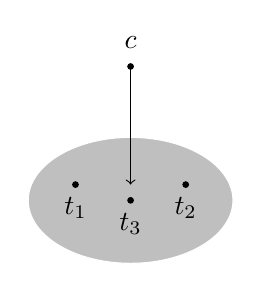
\begin{tikzpicture}
        \filldraw (0, 1.5) circle (1pt);
        \node at (0, 1.8) {$c$};

        \filldraw[fill=gray!50, draw=white] (0, -0.2) ellipse (1.3 and 0.8);
        \filldraw (-0.7, 0) circle (1pt);
        \node at (-0.7, -0.3) {$t_1$};
        \filldraw (0.7, 0) circle (1pt);
        \node at (0.7, -0.3) {$t_2$};
        \filldraw (0, -0.2) circle (1pt);
        \node at (0, -0.5) {$t_3$};

        \draw[->] (0, 1.5) -- (0, 0);
    \end{tikzpicture}
\]

在余完备范畴中,我们总能构造一个余积 $\coprod_{i \in I} t_i$。这个余积是一个弱终端对象,因为有一条从每个 $c$ 到它的箭头。这个箭头是到某个 $t_i$ 的箭头与注入 $\iota_i \colon t_i \to \coprod_{j \in I} t_j$ 的复合。

给定一个弱终端对象,我们可以构造(强)终端对象。我们首先定义 $\cat C$ 的子范畴 $\cat T$,其对象是 $t_i$。$\cat T$ 中的态射是 $\cat C$ 中所有在 $\cat T$ 的对象之间的态射。这称为 $\cat C$ 的\emph{满子范畴(full subcategory)}。通过我们的构造,$\cat T$ 是小范畴。

有一个显然的包含函子 $F$ 将 $\cat T$ 嵌入 $\cat C$。这个函子在 $\cat C$ 中定义了一个小图。事实证明,这个图的余极限是 $\cat C$ 中的终端对象。

对偶地,类似的构造可以用来定义一个弱初对象的极限作为初对象。

这个解集的属性在弗雷德的伴随函子定理的证明中将很有用。

\section{The Yoneda Lemma 延达引理}

从某个范畴 $\mathcal{C}$ 到集合范畴的函子可以被视为该范畴在 $\mathbf{Set}$ 中的模型。建模通常是一个有损过程:它丢弃了一些信息。常值 $\Set$ 函子是一个极端的例子:它将整个范畴映射到单个集合及其恒等函数。

同态函子产生了从某个视角看范畴的模型。函子 $\mathcal{C}(a, -)$,例如,提供了从 $a$ 的视角看 $\mathcal{C}$ 的全景,非常详细。它将所有从 $a$ 发出的箭头组织成整齐的包,连接它们的箭头是按照源范畴的原始结构进行的。

\[
    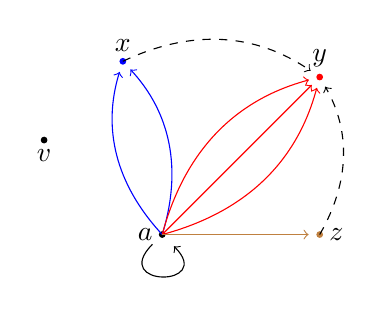
\begin{tikzpicture}
        \def\ax{0}
        \def\ay{0.5}
        \def\xx{-0.5}
        \def\xy{2.7}
        \def\yx{2}
        \def\yy{2.5}
        \def\zx{2}
        \def\zy{0.5}
        \def\vx{-1.5}
        \def\vy{1.7}
        \filldraw[black] (\ax, \ay) circle (1 pt);
        \node (a) at (\ax, \ay) {};
        \node[left] at (\ax, \ay) {$a$};
        \filldraw[blue] (\xx, \xy) circle (1 pt);
        \node[above] at (\xx, \xy) {$x$};
        \filldraw[red] (\yx, \yy) circle (1 pt);
        \node[above] at (\yx, \yy) {$y$};
        \filldraw[brown] (\zx, \zy) circle (1 pt);
        \node[right] at (\zx, \zy) {$z$};
        \filldraw[black] (\vx, \vy) circle (1 pt);
        \node[below] at (\vx, \vy) {$v$};

        \draw [->] (a) edge[out=225, in=315, loop] (a);

        \draw[dashed] (\xx, \xy) edge[->, bend left, shorten > = 4 pt] (\yx, \yy);
        \draw[dashed] (\zx, \zy) edge[->, bend right, shorten > = 4 pt] (\yx, \yy);

        \draw[blue] (\ax, \ay) edge[->, bend left, shorten > = 4 pt] (\xx, \xy);
        \draw[blue] (\ax, \ay) edge[->, bend right, shorten > = 4 pt] (\xx, \xy);

        \draw[red] (\ax, \ay) edge[->, bend left, shorten > = 4 pt] (\yx, \yy);
        \draw[red] (\ax, \ay) edge[->, bend right, shorten > = 4 pt] (\yx, \yy);
        \draw[red] (\ax, \ay) edge[->, shorten > = 4 pt] (\yx, \yy);

        \draw[brown] (\ax, \ay) edge[->, shorten > = 4 pt] (\zx, \zy);
    \end{tikzpicture}
    \hspace{80pt}
    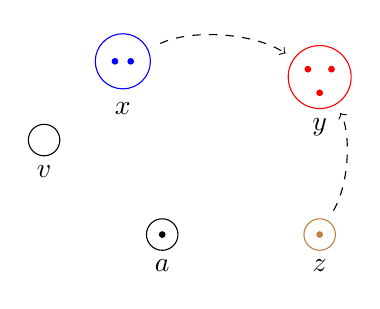
\begin{tikzpicture}
        \def\ax{0}
        \def\ay{0.5}
        \def\xx{-0.5}
        \def\xy{2.7}
        \def\yx{2}
        \def\yy{2.5}
        \def\zx{2}
        \def\zy{0.5}
        \def\vx{-1.5}
        \def\vy{1.7}
        \def\sx{0.7}
        \def\sy{1.6}

        \node at (\sx, \sy) {$\Set$};

        \draw[black] (\vx, \vy) circle (0.2);
        \node[below] at (\vx, \vy - 0.2) {$v$};

        \draw[black] (\ax, \ay) circle (0.2);
        \filldraw[black] (\ax, \ay) circle (1 pt);
        \node[below] at (\ax, \ay-0.2) {$a$};

        \draw[blue] (\xx, \xy) circle (0.35);
        \filldraw[blue] (\xx - 0.1, \xy) circle (1 pt);
        \filldraw[blue] (\xx + 0.1, \xy) circle (1 pt);
        \node[above] at (\xx, \xy - 0.8) {$x$};

        \draw[red] (\yx, \yy) circle (0.4);
        \filldraw[red] (\yx-0.15, \yy+0.1) circle (1 pt);
        \filldraw[red] (\yx+0.15, \yy+0.1) circle (1 pt);
        \filldraw[red] (\yx, \yy-0.2) circle (1 pt);
        \node[below] at (\yx, \yy - 0.4) {$y$};

        \draw[brown] (\zx, \zy) circle (0.2);
        \filldraw[brown] (\zx, \zy) circle (1 pt);
        \node[below] at (\zx, \zy - 0.2) {$z$};

        \draw[dashed] (\xx, \xy) edge[->, bend left, shorten > = 15, shorten < = 15] (\yx, \yy);
        \draw[dashed] (\zx, \zy) edge[->, bend right, shorten > = 15, shorten < = 10] (\yx, \yy);

    \end{tikzpicture}
\]

一些视角比其他视角更好。例如,从初始对象的视角看,景色相当稀疏。每个对象 $x$ 都被映射到单集合 $\cat C(0, x)$,对应于唯一的映射 $0 \to x$。

从终端对象的视角看,则更有趣:它将所有对象映射到其全局元素集合 $\cat C(1, x)$。

延达引理可以被视为范畴论中最深刻的陈述之一,也可以被视为最平凡的陈述之一。让我们从深刻的版本开始。

考虑两个 $\mathcal{C}$ 在 $\mathbf{Set}$ 中的模型。第一个模型由同态函子 $\mathcal{C}(a, -)$ 给出。这是从 $a$ 的视角看到的 $\mathcal{C}$ 的全景、非常详细的视角。第二个模型由某个任意函子 $F \colon \mathcal{C} \to \mathbf{Set}$ 给出。任何这两个模型之间的自然变换都嵌入了一个模型到另一个模型中。事实证明,所有这些自然变换的集合完全由集合 $F a$ 决定。

由于自然变换的集合是函子范畴 $[\mathcal{C}, \mathbf{Set}]$ 中的同态集,延达引理的正式陈述形式如下:

\[ [\mathcal{C}, \mathbf{Set}]( \mathcal{C}(a, -), F) \cong F a \]
此外,这个同构在 $a$ 和 $F$ 上都是自然的。

这种情况之所以成立,是因为这个定理中涉及的所有映射都必须保持 $\mathcal{C}$ 范畴的结构和它们模型的结构。特别是,自然性条件对自然变换的各个分量从一个点传播到另一个点的方式施加了大量约束。

延达引理的证明从单个恒等箭头开始,让自然性在整个范畴中传播。

以下是证明的概述。它分为两部分:首先,给定一个自然变换,我们构造一个 $F a$ 的元素。其次,给定一个 $F a$ 的元素,我们构造相应的自然变换。

首先,让我们选择延达引理左侧的一个任意元素:一个自然变换 $\alpha$。它在 $x$ 处的分量是一个函数:
\[ \alpha_x \colon \mathcal{C}(a, x) \to F x \]
现在我们可以应用延达技巧:用 $a$ 替代 $x$:
\[ \alpha_a \colon \mathcal{C}(a, a) \to F a \]
然后选择 $\mathcal{C}(a, a)$ 的典型元素 $id_a$。结果是集合 $F a$ 中的一个元素 $\alpha_a (id_a)$。这定义了从自然变换到集合 $F a$ 元素的映射。

现在来看另一种情况。给定集合 $F a$ 的一个元素 $p$,我们想要构造一个自然变换 $\alpha$。首先,我们将 $p$ 赋值为 $\alpha_a$ 在 $id_a \in \cat C(a, a)$ 上的作用。

\[
    \begin{tikzpicture}
        \def\ax{0}
        \def\ay{0.5}
        \def\xx{-0.5}
        \def\xy{3.7}
        \filldraw[black] (\ax, \ay) circle (1 pt);
        \node (a) at (\ax, \ay) {};
        \node[left] at (\ax, \ay) {$a$};
        \filldraw[blue] (\xx, \xy) circle (1 pt);
        \node[above] at (\xx, \xy) {$x$};

        \draw [->] (a) edge[out=225, in=315, loop] (a);
        \node[right] at (\ax + 0.3, \ay - 0.35) {$id_a$};

        \draw[blue] (\ax, \ay) edge[->, "$h$", bend right, shorten > = 4 pt] (\xx, \xy);

    \end{tikzpicture}
    \hspace{80pt}
    \begin{tikzpicture}

        \def\ax{0}
        \def\ay{0.5}
        \def\xx{-0.5}
        \def\xy{3.7}

        \def\fax{3}
        \def\fay{0.5}
        \def\fxx{3 - 0.5}
        \def\fxy{3.7}

        \def\px{\fax - 0.3}
        \def\hx{\xx + 0.35}
% C(a,a)
        \draw[black] (\ax, \ay) circle (0.2);
        \filldraw[black] (\ax, \ay) circle (1 pt);
        \node[below] at (\ax, \ay-0.2) {$\cat C (a, a)$};
% C(a,x)
        \draw[black] (\xx, \xy) ellipse (0.7 and 0.4);

        \filldraw[blue] (\xx + 0.35, \xy) circle (1 pt);
        \node[left, blue] at (\hx, \xy) {$h$};

        \node[above] at (\xx, \xy - 1.1) {$\cat C (a, x)$};
        \draw[dashed] (\hx, \xy) edge[->, "$\alpha_x$", shorten > = 4 pt] (\fxx, \fxy);

% F a
        \draw[red] (\fax, \fay) ellipse (0.7 and 0.4);
        \filldraw[red] (\px, \fay) circle (1 pt);
        \node[right, red] at (\px, \fay) {$p$};
        \node[right, red] at (\fax + 0.7, \fay) {$F a$};
        \draw[dashed] (\ax, \ay) edge[->, "$\alpha_a$", shorten > = 3 pt] (\px, \fay);
% F x
        \draw[red] (\fxx, \fxy) circle (0.4);
        \filldraw[red] (\fxx, \fxy) circle (1 pt);
        \node[right, red] at (\fxx + 0.35, \fxy) {$F x$};

        \draw[blue] (\px, \fay) edge[->, "$F h$", bend right, shorten > = 12, shorten < = 12] (\fxx, \fxy);

    \end{tikzpicture}
\]

现在让我们选择一个任意的对象 $x$ 和 $\cat C(a, x)$ 的一个任意元素。后者是一个箭头 $h \colon a \to x$。我们的自然变换必须将其映射到 $F x$ 的一个元素。我们可以通过使用 $F$ 提升箭头 $h$ 来完成此操作。我们得到一个函数:
\[F h \colon F a \to F x \]
我们可以将此函数应用于 $p$ 并得到 $F x$ 的一个元素。我们将这个元素作为 $\alpha_x$ 在 $h$ 上的作用:
\[ \alpha_x h = (F h) p \]

延达引理中的同构在 $a$ 和 $F$ 上都是自然的。后者意味着你可以通过在函子范畴中的箭头,即自然变换,从函子 $F$ ``移动''到另一个函子 $G$。这是抽象水平上的一次飞跃,但在函子范畴中,定义的函子性和自然性都同样适用,其中对象是函子,箭头是自然变换。

\begin{exercise}
    补充证明中的缺口,当 $F a$ 为空时。
\end{exercise}
\begin{exercise}
    证明上述定义的
    \[ \mathcal{C}(a, x) \to F x\]
    的映射是自然变换。提示:使用一些 $f \colon x \to y$ 变换 $x$。
\end{exercise}
\begin{exercise}
    证明公式 $\alpha_x$ 可以从假设 $\alpha_a (id_a) = p$ 和自然性条件中推导出来。提示:同态函子 $\cat C(a, h)$ 的提升由后组成给出。
\end{exercise}

\subsection{Yoneda lemma in programming 延达引理在编程中的应用}

现在来谈论平凡部分:延达引理的证明直接翻译为 Haskell 代码。我们从函子 \hask{a->x} 和某些函子 \hask{f} 之间的自然变换的类型开始,表明它等同于 \hask{f} 在 \hask{a} 上的作用类型。
\begin{haskell}
    forall x. (a -> x) -> f x.   -- is isomorphic to (f a)
\end{haskell}
我们使用标准的延达技巧生成一个类型为 \hask{(f a)} 的值:
\begin{haskell}
    yoneda :: Functor f => (forall x. (a -> x) -> f x) -> f a
    yoneda g = g id
\end{haskell}
以下是反向映射:
\begin{haskell}
    yoneda_1 :: Functor f => f a -> (forall x. (a -> x) -> f x)
    yoneda_1 y = \h -> fmap h y
\end{haskell}

注意,我们通过混合类型和集合有点作弊。目前的延达引理以 $\mathbf{Set}$ 值函子形式工作。同样,正确的表述是,我们使用了在自我扩充范畴中的延达引理扩展版本。

延达引理在编程中有一些有趣的应用。例如,让我们考虑当我们将延达引理应用于恒等函子时会发生什么。我们得到类型 \hask{a}(恒等函子在 \hask{a} 上的作用)和
\begin{haskell}
    forall x. (a -> x) -> x
\end{haskell}
的同构。
我们将其解释为:任何数据类型 \hask{a} 都可以被替换为一个高阶多态函数。这个函数接受另一个函数——称为处理器、回调或\emph{延续(continuation)}——作为参数。

这是标准的延续传递变换,在分布式编程中使用很多,例如当类型 \hask{a} 的值必须从远程服务器检索时。它也可以作为一种程序变换,用于将递归算法转化为尾递归函数。

延续传递风格难以使用,因为延续的组合非常复杂,程序员通常称之为``回调地狱''。幸运的是,延续形成了一个单子,这意味着它们的组合可以隐藏在 \hask{do} 记法背后。

\subsection{The contravariant Yoneda lemma 反变延达引理}

通过反转几个箭头,延达引理也可以应用于反变函子。它适用于反变同态函子 $\mathcal{C}(-, a)$ 和反变函子 $F$ 之间的自然变换:

\[ [\mathcal{C}^{op}, \mathbf{Set}]( \mathcal{C}(-, a), F) \cong F a \]

这是映射的 Haskell 实现:
\begin{haskell}
    coyoneda :: Contravariant f => (forall x. (x -> a) -> f x) -> f a
    coyoneda g = g id
\end{haskell}
这是逆变换:
\begin{haskell}
    coyoneda_1 :: Contravariant f => f a -> (forall x. (x -> a) -> f x)
    coyoneda_1 y = \h -> contramap h y
\end{haskell}

\section{Yoneda Embedding(Yoneda 嵌入)}

在封闭范畴(closed category)中,我们有指数对象(exponential objects),它们可以作为同态集(hom-sets)的代表。在$\Set$中,同态集本身就是集合,因此它们自动成为$\Set$中的对象。

另一方面,在范畴的范畴(category of categories)$\mathbf{Cat}$中,同态集是函子(functors)的集合,并不是一开始就显而易见它们可以提升为$\mathbf{Cat}$中的对象——即一个范畴。但如我们之前所见,它们确实可以!任意两个范畴之间的函子形成了一个函子范畴(functor category)。

因此,我们可以像柯里化函数那样柯里化函子。从积范畴(product category)到另一个范畴的函子可以看作返回一个函子的函子。换句话说,$\mathbf{Cat}$是一个封闭的(对称的)单体范畴(monoidal category)。

特别地,我们可以对同态函子$\mathcal{C}(a, b)$进行柯里化。它是一个跨积范畴的伴随函子(profunctor),或者说是从积范畴到$\mathbf{Set}$的函子:
$$\mathcal{C}^{op} \times \mathcal{C} \to  \mathbf{Set}$$
但它在第一个参数$a$上也是一个逆变函子(contravariant functor)。对于$\mathcal{C}^{op}$中的每个$a$,它生成一个协变函子(covariant functor)$\mathcal{C}(a, -)$,这是函子范畴$[\mathcal{C}, \mathbf{Set}]$中的一个对象。我们可以将这个映射写为:
$$\mathcal{C}^{op} \to [\mathcal{C},  \mathbf{Set}]$$
或者,我们可以固定$b$并生成一个逆变函子$\mathcal{C}(-, b)$。这个映射可以写成:
$$\mathcal{C} \to [\mathcal{C}^{op},  \mathbf{Set}]$$
这两个映射都是函子性的,这意味着,例如,$\mathcal{C}$中的一个箭头会被映射为$[\mathcal{C}^{op},  \mathbf{Set}]$中的一个自然变换(natural transformation)。

这些$\mathbf{Set}$值函子范畴很常见,以至于它们有特别的名称。$[\mathcal{C}^{op},  \mathbf{Set}]$中的函子被称为\emph{presheaves}(预层),而$[\mathcal{C},  \mathbf{Set}]$中的函子被称为\emph{co-presheaves}(对预层)。(这些名称来自代数拓扑。)

让我们重点关注以下对同态函子的解释:
$$\mathcal{Y} \colon \mathcal{C} \to [\mathcal{C}^{op},  \mathbf{Set}]$$
它接受一个对象$x$并将其映射为一个预层
$$\mathcal{Y}_x = \mathcal{C}(-, x)$$
这可以被视为从所有可能方向对$x$的全部视图的集合。

让我们也回顾一下它对箭头的作用。函子$\mathcal{Y}$将箭头$f \colon x \to y$提升为预层之间的映射:
$$\alpha \colon \mathcal{C}(-, x) \to \mathcal{C}(-, y)$$
这个自然变换在某个$z$上的分量是同态集之间的一个函数:
$$\alpha_z \colon \mathcal{C}(z, x) \to \mathcal{C}(z, y)$$
这简单地通过后合成(post-composition)$(f \circ -)$来实现。

这样的函子$\mathcal{Y}$可以被认为是在预层范畴中创建了一个$\mathcal{C}$的模型。但这不是一个普通的模型——它是一个将一个范畴嵌入到另一个范畴中的\emph{嵌入}(embedding)。这个特定的嵌入被称为\emph{Yoneda embedding(Yoneda 嵌入)},而函子$\mathcal{Y}$被称为\emph{Yoneda functor(Yoneda 函子)}。

首先,$\mathcal{C}$的每个对象都被映射为$[\mathcal{C}^{op}, \mathbf{Set}]$中的一个\emph{不同的}对象(预层)。我们说它是\emph{对象上的单射}(injective on objects)。

但这还不是全部:$\mathcal{C}$中的每个箭头都被映射为一个\emph{不同的}箭头。我们说这个嵌入函子是\emph{忠实的函子}(faithful functor)。

如果这还不够,映射同态集的过程也是\emph{满射的}(surjective),这意味着$[\mathcal{C}^{op},  \mathbf{Set}]$中对象之间的每个箭头都来自$\mathcal{C}$中的某个箭头。我们说这个函子是\emph{充满函子}(full functor)。

总而言之,这个嵌入是\emph{完全忠实的}(fully faithful),即箭头的映射是一一对应的。然而,一般来说,Yoneda 嵌入在对象上并\emph{不}是满射的,因此称为“嵌入”。

这个嵌入完全忠实的事实是Yoneda 引理的直接结果。实际上,我们知道,对于任意函子$F \colon \mathcal{C}^{op} \to \mathbf{Set}$,我们有一个自然同构:
$$[\mathcal{C}^{op}, \mathbf{Set}](\mathcal{C}(-, x), F) \cong F x$$
特别地,我们可以将另一个同态函子$\mathcal{C}(-, y)$替换为$F$,得到:
$$[\mathcal{C}^{op}, \mathbf{Set}](\mathcal{C}(-, x), \mathcal{C}(-, y)) \cong \mathcal{C}(x, y)$$
左侧是预层范畴中的同态集,而右侧是$\mathcal{C}$中的同态集。它们是同构的,这证明了嵌入是完全忠实的。事实上,Yoneda 引理告诉我们,这个同构在$x$和$y$中是自然的。

让我们仔细看看这个同构。让我们选择右侧集合$\mathcal{C}(x, y)$的一个元素——一个箭头$f \colon x \to y$。这个同构将它映射为一个自然变换,其在$z$上的分量是一个函数:
$$\mathcal{C}(z, x) \to \mathcal{C}(z, y)$$
这个映射通过后合成$(f \circ -)$实现。

在Haskell中,我们会这样写:
\begin{haskell}
    toNatural :: (x -> y) -> (forall z. (z -> x) -> (z -> y))
    toNatural f = \h -> f . h
\end{haskell}
事实上,这种语法也有效:
\begin{haskell}
    toNatural f = (f . )
\end{haskell}
反向映射是:
\begin{haskell}
    fromNatural :: (forall z. (z -> x) -> (z -> y)) -> (x -> y)
    fromNatural alpha = alpha id
\end{haskell}
(再次注意使用了Yoneda技巧。)

这个同构将恒等映射为恒等,并将组合映射为组合。因为它是通过后合成实现的,而后合成保持了恒等和组合。我们在同构一章中已经展示过这个事实:
$$((f \circ g) \circ -) = (f \circ -) \circ (g \circ -)$$

因为它保持了组合和恒等,这个同构也保持了\emph{同构}(isomorphisms)。所以,如果$x$和$y$是同构的,那么预层$\mathcal{C}(-, x)$和$\mathcal{C}(-, y)$也是同构的,反之亦然。

我们在之前各章中一直使用这个结果来证明许多同构。如果同态集自然同构,那么对象也是同构的。

Yoneda 嵌入建立在这样一种思想之上,即一个对象与其他对象的关系决定了这个对象的一切。预层$\cat C (-, a)$,就像一个全息图,编码了从整个范畴$\cat C$的角度看$a$的所有视图。Yoneda

嵌入告诉我们,当我们将这些单独的全息图结合起来时,我们得到了整个范畴的完美全息图。

\section{Representable Functors(可表函子)}

对预层范畴中的对象是将集合分配给$\mathcal{C}$中的对象的函子(functors)。其中一些函子通过选择一个参考对象$a$来工作,并将所有对象$x$映射为它们的同态集$\mathcal{C}(a, x)$:
$$F x = \cat C(a, x)$$
这样的函子以及所有与之同构的函子称为\emph{representable(可表函子)}。整个函子由单个对象$a$来“表示”。

在封闭范畴中,将每个对象$x$映射为指数对象$x^a$的元素集合的函子由$a$表示。这是因为$x^a$的元素集合同构于$\mathcal{C}(a, x)$:
$$\mathcal{C}(1, x^a) \cong \mathcal{C}(1 \times a, x) \cong \mathcal{C} (a, x)$$

从这个角度看,表示对象$a$就像是一个函子的对数。

这个类比更深入:正如乘积的对数是对数之和一样,乘积数据类型的表示对象是一个和。例如,使用乘积平方其参数的函子$F x = x \times x$由$2$表示,这是和$1 + 1$。实际上,我们之前已经看到$x \times x \cong x^2$。

可表函子在$\mathbf{Set}$值函子的范畴中扮演着非常特殊的角色。注意到Yoneda 嵌入将$\mathcal{C}$的所有对象映射为可表预层。它将一个对象$x$映射为由$x$表示的预层:
$$\mathcal{Y} \colon x \mapsto \mathcal{C}(-, x)$$

我们可以在预层范畴中找到整个范畴$\mathcal{C}$,对象和态射都嵌入为可表函子。问题是,在可表函子之间,预层范畴中还有什么“在它们之间”呢?

就像有理数在实数中是稠密的,可表函子在(对)预层中也是“稠密的”。每个实数可以通过有理数逼近。每个预层都是可表函子的上极限(colimit)(而每个对预层则是下极限(limit))。我们将在讨论(对)端点(ends)时回到这个话题。

\begin{exercise}
    描述作为表示对象的极限和上极限。它们表示什么样的函子?
\end{exercise}
\begin{exercise}
    考虑一个\emph{singleton functor(单例函子)}$F \colon \cat C \to \Set$,它将每个对象$c$映射为仅包含该对象的单例集合$\{c\}$(即,每个对象有不同的单例集合)。定义$F$对箭头的作用。证明$F$是可表的等价于$\cat C$有一个初始对象(initial object)。
\end{exercise}

\subsection{The guessing game(猜谜游戏)}

通过一个假想的猜谜游戏,有时可以说明对象如何通过与其他对象的相互作用来描述。一个范畴理论家在一个范畴中选择一个秘密对象,而另一个人则必须猜出它是什么(当然,是同构的)。

猜测者可以指向对象,并使用它们作为探测秘密对象的“探针”。对手每次都应以一个集合作为回应:从探测对象$a$到秘密对象$x$的箭头集合。这当然就是同态集$\mathcal{C}(a, x)$。

这些答案的总和,只要对手没有作弊,将定义一个预层$F \colon \mathcal{C}^{op} \to \mathbf{Set}$,他们隐藏的对象就是它的表示对象。

但我们怎么知道第二个范畴理论家没有作弊呢?为了验证这一点,我们询问关于箭头的问题。对于我们选择的每个箭头,他们应该给我们两个集合之间的一个函数——他们为其端点给出的集合。我们可以检查所有恒等箭头是否被映射为恒等函数,组合的箭头是否映射为函数的组合。换句话说,我们将能够验证$F$确实是一个函子。

然而,一个足够聪明的对手可能仍然会欺骗我们。他们揭示给我们的预层可能描述了一个幻想的对象——他们的想象的产物——而我们却无法辨别。事实证明,这样的幻想物体往往与真实物体一样有趣。

\subsection{Representable functors in programming(编程中的可表函子)}

在Haskell中,我们使用两个函数定义了一个可表函子类,它们见证了这个同构:
$$F x = \cat C(a, x)$$
第一个函数,\hask{tabulate},将一个函数转换为查找表;第二个函数,\hask{index},使用表示类型\hask{Key}来索引它。

\begin{haskell}
    class Representable f where
    type Key f :: Type
    tabulate :: (Key f -> x) -> f x
    index    :: f x -> (Key f -> x)
\end{haskell}

使用和(sum)的代数数据类型不可表示(没有公式可以取和的对数)。例如,列表类型被定义为一个和,因此它不可表示。然而,无限流是可表示的。

从概念上讲,流就像一个无限元组,技术上来说是一个积。这种流由自然数类型表示。换句话说,一个无限流等价于自然数的映射。
\begin{haskell}
    data Stream a = Stm a (Stream a)
\end{haskell}
下面是实例定义:
\begin{haskell}
    instance Representable Stream where
    type Key Stream = Nat
    tabulate g = tab Z
    where
    tab n = Stm (g n) (tab (S n))
    index stm = \n -> ind n stm
    where
    ind Z (Stm a _) = a
    ind (S n) (Stm _ as) = ind n as
\end{haskell}
可表类型对于实现\emph{memoization(记忆化)}函数非常有用。

\begin{exercise}
    为\hask{Pair}实现\hask{Representable}实例:
    \begin{haskell}
        data Pair x = Pair x x
    \end{haskell}
\end{exercise}

\begin{exercise}
    将所有内容映射为终端对象的常量函子是可表的么?提示:1的对数是什么?

    在Haskell中,这样的函子可以实现为:
    \begin{haskell}
        data Unit a = U
    \end{haskell}
    为其实现\hask{Representable}实例。
\end{exercise}

\begin{exercise}
    列表函子不可表示。但它可以被认为是可表的和吗?
\end{exercise}

\section{2-category  $\mathbf{Cat}$ (2-范畴 $\mathbf{Cat}$)}

在范畴的范畴$\mathbf{Cat}$中,同态集不仅仅是集合。每个同态集都可以提升为一个函子范畴,其中自然变换(natural transformations)扮演箭头的角色。这种结构被称为2-范畴(2-category)。

在2-范畴的语言中,对象称为\emph{0-cells}(0-胞元),它们之间的箭头称为\emph{1-cells}(1-胞元),而箭头之间的箭头称为\emph{2-cells}(2-胞元)。

这一图景的明显推广是,在2-胞元之间有3-胞元,依此类推。一个\emph{$n$-category}($n$-范畴)有一直到第$n$层的胞元。

但为什么不让箭头一直延伸呢?这就引出了\emph{infinity categories($\infty$-范畴)}。远非一种好奇心,$\infty$-范畴在实际应用中有其用途。例如,它们在代数拓扑中用于描述点、点之间的路径、路径扫过的曲面、曲面扫过的体积,依此类推,直到无穷。

\section{Useful Formulas(实用公式)}
\begin{itemize}
    \item 对协变函子的Yoneda 引理:
    $$[\mathcal{C}, \mathbf{Set}](\mathcal{C}(a, -), F) \cong F a$$
    \item 对逆变函子的Yoneda 引理:
    $$[\mathcal{C}^{

        op}, \mathbf{Set}](\mathcal{C}(-, a), F) \cong F a$$
    \item Yoneda 引理的推论:
    \begin{align*}
    [\mathcal{C}, \mathbf{Set}](\mathcal{C}(x, -), \mathcal{C}(y, -)) &\cong \mathcal{C}(y, x) \\
    [\mathcal{C}^{op}, \mathbf{Set}](\mathcal{C}(-, x), \mathcal{C}(-, y)) &\cong \mathcal{C}(x, y)
    \end{align*}
\end{itemize}

\end{document}